% https://tex.stackexchange.com/a/146410
\documentclass{beamer}

\usepackage{tikz}
\usetikzlibrary{arrows}
\tikzset{
    treenode/.style = {align=center, inner sep=0pt, text centered,
        font=\sffamily},
    arn_n/.style = {treenode, circle,black, draw=black, text width=1.3em}% 
}

\begin{document}
    \begin{frame} 
        \frametitle{Paragraphs of Text}
        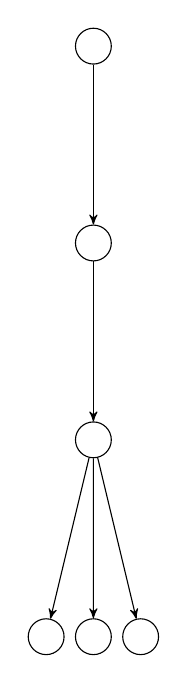
\begin{tikzpicture}[
            ->,
            >=stealth',
            level distance = 2.5cm,
            level 1/.style={sibling distance=5.75cm},
            level 2/.style={sibling distance=1.95cm},
            level 3/.style={sibling distance=0.6cm}
            ] 
            \node [arn_n] {}
            child{ 
                node [arn_n] {} 
                child{ node [arn_n] {} 
                    child{ node [arn_n] {} }
                    child{ node [arn_n] {} }
                    child{ node [arn_n] {} }
                }
            }; 
        \end{tikzpicture}
    \end{frame}
\end{document}
